\chapter{Analisis}
\label{chap:analisis}

Bab ini terdiri atas lima bagian, yaitu Analisis Google Authentication, Analisis Markdown, Analisis StrapdownJS, Analisis Zurb dan Analisis Berorientasi Objek. Bagian Analisis Google Authentication berisi penjelasan analisis Google Authentication yang akan digunakan pada penelitian ini. Bagian Analisis Markdown berisi penjelasan analisis Markdown yang akan digunakan pada penelitian ini. Bagian Analisis StrapdownJS berisi penjelasan analisis StrapdownJS yang akan digunakan pada penelitian ini. Bagian Analisis Zurb Foundation berisi penjelasan analisis Zurb Foundation yang akan digunakan pada penelitian ini. Sedangkan bagian Analisi Berorientasi Objek berisi use case diagram dan skenario perangkat lunak yang akan dibangun.

\section{Analisis Google Authentication}
\label{sec:analisisGoogleAuthentication}

Peda penelitian ini untuk otentikasi fitur login akan menggunakan teknologi Google authentication atau dikenal OAuth 2.0. Untuk langkah-langkah penggunaan OAuth 2.0 dapat dilihat pada sub bab berikutnya.

\subsection{Langkah Dasar Penggunaan OAuth 2.0}
Berdasarkan langkah dasar yang terdapat pada bab 2, maka terdapat empat langkah yang akan diikuti untuk menggunakan OAuth 2.0 pada penelitian ini. Empat langkah yang diikuti:
\begin{enumerate}
\item Mendapatkan kepercayaan OAuth 2.0 dari Google Developers Console\\
    \begin{enumerate}
    \item Mengunjungi Google Developers Console. Agar lebih jelas dapat dilihat pada Gambar \ref{fig:gdc}.
    \item Buat sebuah proyek baru. Dapat dilihat pada Gambar \ref{fig:newproject}.
    \item Masuk ke proyek yang telah dibuat dan masuk ke menu 'Credentials'. Agar lebih jelas dapat dilihat pada Gambar \ref{fig:credentials}.
    \item Membuat client ID yang baru. Dapat dilihat pada Gambar \ref{fig:newclientid}.
    \item Pilih tipe aplikasi sesuai aplikasi yang dibangun, pada penelitian ini menggunakan tipe aplikasi web karena aplikasi yang akan dibangun berbasis web. Agar lebih jelas dapat dilihat pada Gambar \ref{fig:tipeaplikasi}.
    \item Isi bagian AUTHORIZED JAVASCRIPT ORIGINS (merupakan path dimana javasript otorisasi akan dijalankan) pada penelitian ini bagian AUTHORIZED JAVASCRIPT ORIGINS akan diisi dengan http://localhost/ karena aplikasi yang akan dibangun pada penelitian ini terletak pada localhost dan AUTHORIZED REDIRECT URIS (merupakan pengarah jika otorisasi sudah berhasil) pada penelitian ini bagian AUTHORIZED REDIRECT URIS akan diisi dengan http://localhost/pilihmahasiswa.php karena setelah menjalankan aplikasi dan berhasil melakukan otoritasi maka yang halaman pertama yang akan dituju adalah pilihmahasiswa.php. Agar lebih jelas dapat dilihat pada Gambar \ref{fig:tipeaplikasisudahdiisi}.
    \item Setelah langkah-langkah diatas terpenuhi maka akan mendapatkan client id dan client secret. Client id dan client secret yang didapat dapat dilihat di bawah ini.
\begin{lstlisting}
Client id:
568951368854-ufmbistn0pcaq0khubafo1a133orfgve.apps.googleusercontent.com
Client secret:
-cSZ-AUmeQ9PaWWry_IpiBBi
\end{lstlisting}
Agar lebih jelas dapat dilihat pada Gambar \ref{fig:clientid}.
    \end{enumerate}
\item Memperoleh token akses dari Google Authorization Server\\
Untuk memperoleh token akses akan menggunakan izin dari pihak pengguna. Jadi pada saat melakukan login, pengguna diharuskan login menggunakan akun Google sendiri. Setelah login pengguna akan ditanya dan akan memberi respon untuk memberi izin atau tidak pada aplikasi yang telah melakukan permintaan tersebut. Untuk gambar izin dari pihak pengguna dapat dilihat pada Gambar \ref{fig:izinpengguna}.
\item Kirim token ke API\\
Setelah mendapatkan token akses, maka untuk mengirimkan ke API diperlukan scope. Karena sesuai dengan landasan teori, jika token akses dikeluarkan untuk Google+ API maka token akses tersebut tidak berlaku untuk mengakses Google Contact API. Scope yang akan digunakan pada penelitan ini adalah:
\begin{lstlisting}
https://www.googleapis.com/auth/urlshortener
https://www.googleapis.com/auth/userinfo.profile
\end{lstlisting}
\item Memperbaharui token akses jika diperlukan\\
Pada penelitian ini tidak akan menggunakan tahap memperbaharui token akses karena token akses hanya digunakan selama penelitian ini berlangsung.
\end{enumerate}

\begin{figure}[H]
\centering
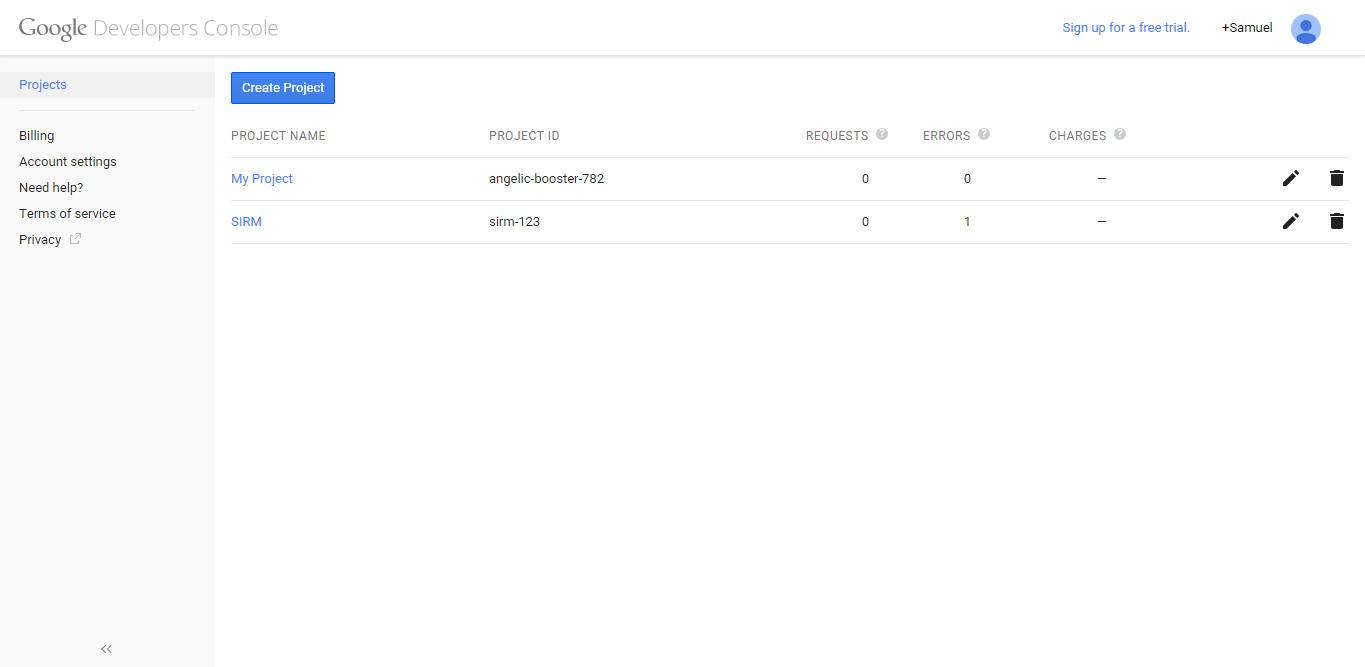
\includegraphics[scale=0.6]{Gambar/GDC.png}
\caption[Google Developers Console]{Google Developers Console} 
\label{fig:gdc}
\end{figure}

\begin{figure}[H]
\centering
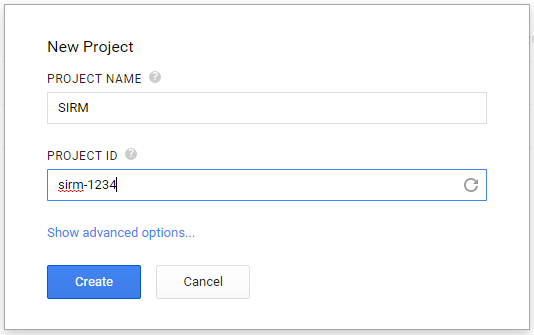
\includegraphics[scale=1]{Gambar/newproject.png}
\caption[Membuat Proyek Baru]{Membuat Proyek Baru} 
\label{fig:newproject}
\end{figure}

\begin{figure}[H]
\centering
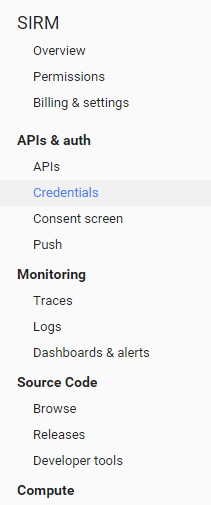
\includegraphics[scale=1]{Gambar/credentials.png}
\caption[Menu Credentials]{Menu Credentials} 
\label{fig:credentials}
\end{figure}

\begin{figure}[H]
\centering
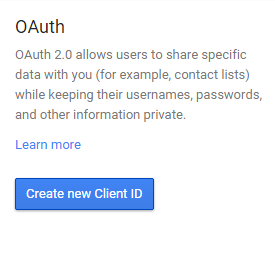
\includegraphics[scale=1]{Gambar/newclientid.png}
\caption[Membuat Client ID yang Baru]{Membuat Client ID yang Baru} 
\label{fig:newclientid}
\end{figure}

\begin{figure}[H]
\centering
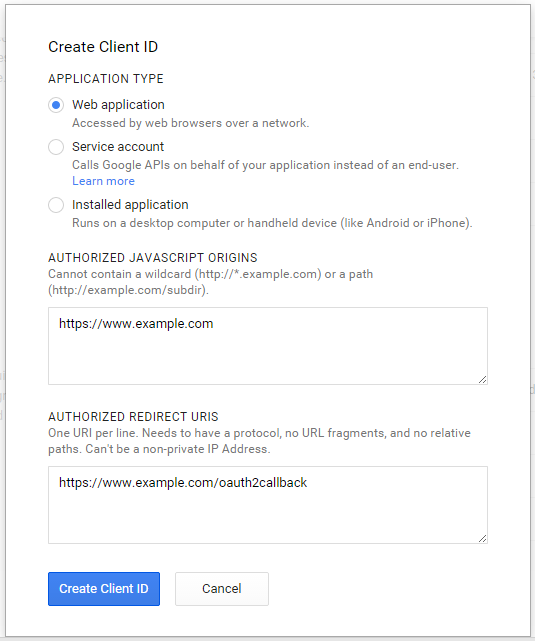
\includegraphics[scale=1]{Gambar/tipeaplikasi.png}
\caption[Tipe Aplikasi]{Tipe Aplikasi} 
\label{fig:tipeaplikasi}
\end{figure}

\begin{figure}[H]
\centering
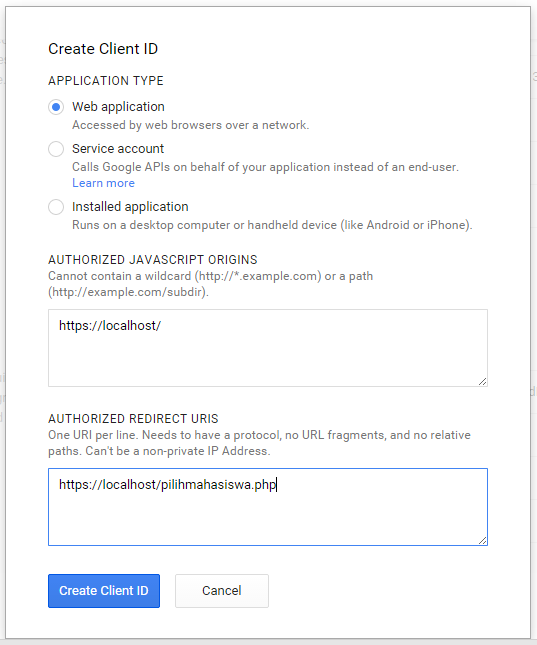
\includegraphics[scale=1]{Gambar/tipeaplikasisudahdiisi.png}
\caption[Pengisian Tipe Aplikasi]{Pengisian Tipe Aplikasi} 
\label{fig:tipeaplikasisudahdiisi}
\end{figure}

\begin{figure}[H]
\centering
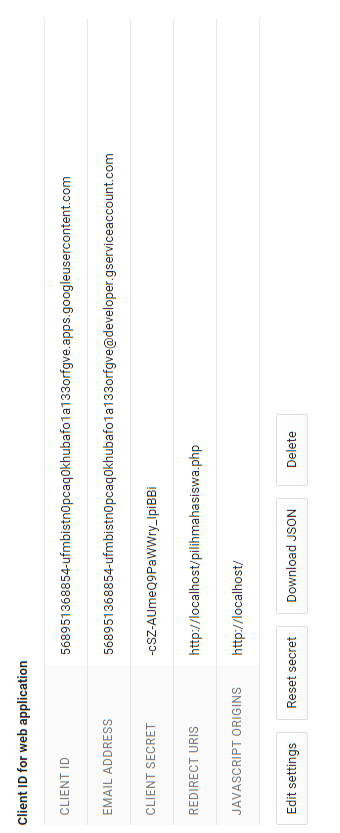
\includegraphics[scale=1]{Gambar/clientid.png}
\caption[Client ID]{Client ID} 
\label{fig:clientid}
\end{figure}

\begin{figure}[H]
\centering
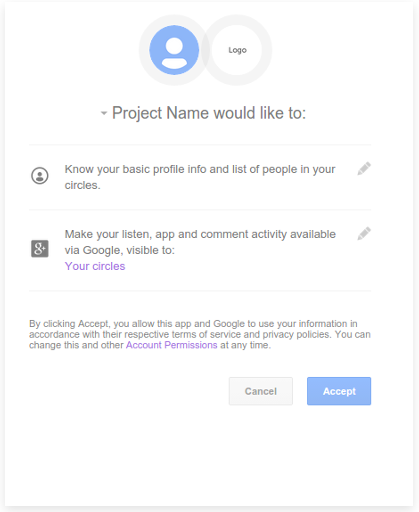
\includegraphics[scale=1]{Gambar/izinpengguna.png}
\caption[Izin Pihak Pengguna]{Izin Pihak Pengguna} 
\label{fig:izinpengguna}
\end{figure}

\subsection{Skenario Aplikasi}
Berdasarkan landasan teori skenario yang ada pada bab 2 dan berdasarkan perangkat lunak yang akan dibangun, maka skenario yang akan digunakan pada penelitian ini adalah skenario aplikasi web server. Aplikasi SIRM akan melakukan permintaan token ke Server Google. Dosen sebagai pengguna akan melakukan login dan memberikan izin. Server Google akan memberikan balasan berupa kode otorisasi. Kemudian aplikasi akan menukarkan kode tersebut untuk mendapatkan token akses. Server Google memberikan token akses sebagai respon penukaran kode otorisasi dengan token akses. Setelah aplikasi mendapatkan token akses, maka apliksi dapat memanggil Google API dengan menggukan token akses. Untuk skenario aplikasi SIRM dapat dilihat pada Gambar \ref{fig:skenarioaplikasisirm}.

\begin{figure}[H]
\centering
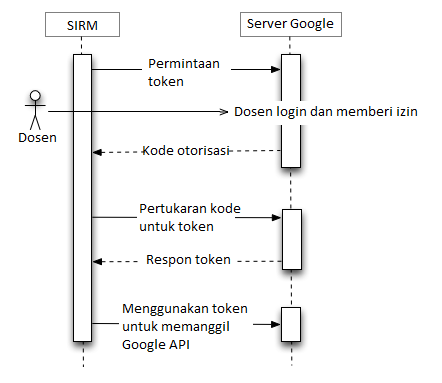
\includegraphics[scale=1]{Gambar/skenarioaplikasisirm.png}
\caption[Skenario Aplikasi SIRM]{Skenario Aplikasi SIRM} 
\label{fig:skenarioaplikasisirm}
\end{figure}

\section{Analisis Markdown}
\label{sec:analisisMarkdown}
Sintaks Markdown yang akan digunakan sesuai dengan landasan teori pada bab 2. Sintaks Markdown akan digunakan pada bagian keterangan mahasiswa agar seragam dalam penulisannya. Keterangan mahasiswa yang akan ditampilkan antara lain; NPM, nama, deskripsi umum, catatan. Maka dari itu sintaks Markdown yang akan digunakan adalah Cetak Tebal dan Cetak Miring, Judul Bab, Batas Baris, Paragraf, Link, dan Daftar.

\begin{itemize}
\item Sintask Cetak Tebal dan Cetak Miring\\
Sintaks ini akan digunakan untuk memberikan penekanan pada satu kata dalam satu kalimat. Berikut penggunaan sintaks dan hasilnya dapat dilihat pada Gambar \ref{fig:cetaktebal}.
\begin{lstlisting}
**NPM** - *2010730013*
\end{lstlisting}
\item Sintaks Judul Bab\\
Sintaks ini akan digunakan untuk menampilkan judul setiap bagian (NPM, nama, umum, dan catatan). Berikut penggunaan sintasks dan hasilnya dapat dilihat pada Gambar \ref{fig:judul}.
\begin{lstlisting}
# Judul 1
## Judul 2
### Judul 3
#### Judul 4
##### Judul 5
###### Judul 6
\end{lstlisting}
\item Sintaks Batas Baris\\
Sintaks ini digunakan pada penulisan paragraf jika diperlukan untuk mengakhiri sebuah baris atau ingin membuat baris baru. Berikut penggunaan sintaks dan hasilnya dapat dilihat pada Gambar \ref{fig:batasbaris}.
\begin{lstlisting}
Baris ini dengan   
batas baris

Baris ini tanpa
batas baris
\end{lstlisting}
\item Sintaks Paragraf\\
Sintaks ini akan digunakan untuk menulis deskripsi umum mahasiswa. Berikut penggunaan sintaks dan hasilnya dapat dilihat pada Gambar \ref{fig:paragraf}.
\begin{lstlisting}
Samuel adalah seorang mahasiswa yang periang namun terkadang sulit diatur. Dia aktif di himpunan sebagai ketua divisi pelayanan masyarakat.

Grady adalah seorang mahasiswa yang memiliki jiwa pemimpin. Dia aktif di UKM  sebagai ketua divisi logistik.
\end{lstlisting}
\item Link\\
Sintaks ini akan digunakan untuk menampilakan website mahasiswa jika mahasiswa yang bersangkutan memiliki sebuah website maupun blog. Berikut penggunaan sintaks dan hasilnya dapat dilihat pada Gambar \ref{fig:link}.
\begin{lstlisting}
Yang bersangkutan memiliki blog di [http://bletack.blogspot.com/](http://bletack.blogspot.com/).
\end{lstlisting}
\item Daftar\\
Sintaks ini akan digunakan untuk menampilkan daftar catatan. Berikut penggunaan sintaks dan hasilnya dapat dilihat pada Gambar \ref{fig:daftar}.
\begin{lstlisting}
* 9 Oktober 2014, bimbingan skripsi
* 3 Oktober 2014, bimbingan skripsi
* 1 September 2014, perwalian
* 1 September 2014, pertama kali dibuat
\end{lstlisting}
\end{itemize}

\begin{figure}[H]
\centering
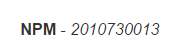
\includegraphics[scale=1]{Gambar/cetaktebal.png}
\caption[Output Sintaks Cetak Tebal dan Cetak Miring]{Output Sintaks Cetak Tebal dan Cetak Miring} 
\label{fig:cetaktebal}
\end{figure}

\begin{figure}[H]
\centering
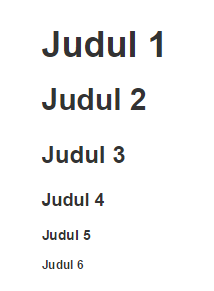
\includegraphics[scale=1]{Gambar/judul.png}
\caption[Output Sintaks Judul Bab]{Output Sintaks Judul Bab} 
\label{fig:judul}
\end{figure}

\begin{figure}[H]
\centering
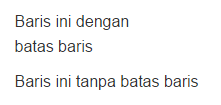
\includegraphics[scale=1]{Gambar/batasbaris.png}
\caption[Output Sintaks Batas Baris]{Output Sintaks Batas Baris} 
\label{fig:batasbaris}
\end{figure}

\begin{figure}[H]
\centering
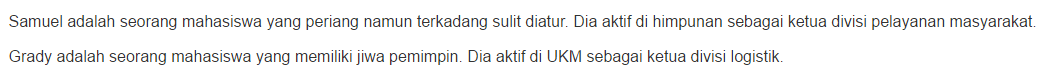
\includegraphics[scale=0.5]{Gambar/paragraf.png}
\caption[Output Sintaks Paragraf]{Output Sintaks Paragraf} 
\label{fig:paragraf}
\end{figure}

\begin{figure}[H]
\centering
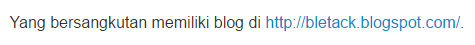
\includegraphics[scale=1]{Gambar/link.png}
\caption[Output Sintaks Link]{Output Sintaks Link} 
\label{fig:link}
\end{figure}

\begin{figure}[H]
\centering
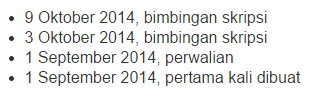
\includegraphics[scale=1]{Gambar/daftar.png}
\caption[Output Sintaks Daftar]{Output Sintaks Daftar} 
\label{fig:daftar}
\end{figure}

Berikut penggunaan sintaks Markdown secara keseluruan untuk bagian keterangan mahasiswa. Berikut penggunaan sintaks dan hasilnya dapat dilihat pada Gambar
\begin{lstlisting}
### NPM

2010730013

### Nama

Samuel
			
### Umum
			
Samuel adalah seorang mahasiswa yang periang namun terkadang sulit diatur. Dia aktif di himpunan sebagai ketua divisi pelayanan masyarakat. Yang bersangkutan memiliki blog di [http://bletack.blogspot.com/](http://bletack.blogspot.com/).
			
### Catatan
			
* 9 Oktober 2014, bimbingan skripsi
* 3 Oktober 2014, bimbingan skripsi
* 1 September 2014, perwalian
* 1 September 2014, pertama kali dibuat
\end{lstlisting}

\begin{figure}[H]
\centering
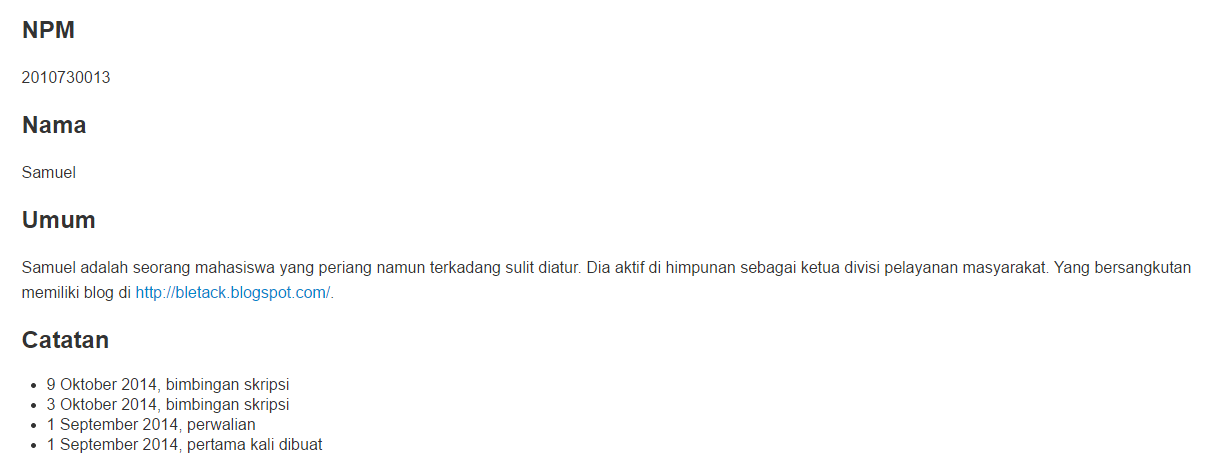
\includegraphics[scale=0.5]{Gambar/overall.png}
\caption[Output Keterangan Mahasiswa]{Output Keterangan Mahasiswa} 
\label{fig:overall}
\end{figure}

\section{Analisis StrapdownJS}
\label{sec:analisisStrapdownJS}
StrapdownJS digunakan untuk menampilkan sintaks Markdown ke halaman HTML. Pada penelitan ini strapdown.js terlebih dahulu diunduh dan untuk menggunakannya menggunakan path seperti di bawah ini.
\begin{lstlisting}
<script src="js/0.2/strapdown.js"></script>
\end{lstlisting}
Skrip tersebut disisipkan pada skrip infomahasiswa.php yang berfungsi untuk menampilkan info mahasiswa yang dimana info tersebut ditulis menggunakan sintaks Markdown. Berikut skrip infomahasiswa.php yang menggunakan strapdown.js.
\begin{lstlisting}
<!doctype html>
<html class="no-js" lang="en">
	<head>
		<meta charset="utf-8" />
		<meta name="viewport" content="width=device-width, initial-scale=1.0" />
		<title>SIRM | Welcome</title>
		<link rel="stylesheet" href="css/foundation.css" />
		<script src="js/vendor/modernizr.js"></script>
	</head>
	<body>
		<div class="row">
			<h5>Anda melihat catatan mahasiswa ini sebagai test@unpar.ac.id.</h5>
		</div>
		<div class="row">
			<ul class="button-group">
				<li><a href="editmahasiswa.php" class="button">Edit</a></li>
				<li><a href="lihathistori.php" class="button">Lihat Histori</a></li>
			</ul>
		</div>
		<hr/>
<xmp style="display:none;">
### NPM

2010730013

### Nama

Samuel
			
### Umum
			
Samuel adalah seorang mahasiswa yang periang namun terkadang sulit diatur. Dia aktif di himpunan sebagai ketua divisi pelayanan masyarakat. Yang bersangkutan memiliki blog di [http://bletack.blogspot.com/](http://bletack.blogspot.com/).
			
### Catatan
			
* 9 Oktober 2014, bimbingan skripsi
* 3 Oktober 2014, bimbingan skripsi
* 1 September 2014, perwalian
* 1 September 2014, pertama kali dibuat

</xmp>
		<script src="js/0.2/strapdown.js"></script>
	</body>
</html>
\end{lstlisting}
Untuk baris 17 sampai baris 37 akan diambil dari database.

\section{Analisis Zurb Foundation}
\label{sec:analisisZurbFoundation}
Zurb Foundation digunakan untuk membuat tampilan antarmuka aplikasi yang akan dibangun. Sesuai landasan teori pada bab 2, pada aplikasi ini menggunakan tiga bagian yaitu Grid, Tabel dan Tombol. Grid digunakan untuk mengatur pembagian tata letak komples sehingga terlihat rapih. Tabel digunakan untuk menampilkan data yang berasal dari database. Tombol digunakan untuk merubah tombol yang biasa menjadi lebih enak untuk dilihat. Berikut sintaks penggunaan Grid, Tabel, dan Tombol pada pilihmahasiswa.php dan untuk gambar dapat dilihat pada Gambar \ref{fig:pilihmahasiswa}.

\begin{lstlisting}
<!doctype html>
<html class="no-js" lang="en">
	<head>
		<meta charset="utf-8" />
		<meta name="viewport" content="width=device-width, initial-scale=1.0" />
		<title>SIRM | Welcome</title>
		<link rel="stylesheet" href="css/foundation.css" />
		<script src="js/vendor/modernizr.js"></script>
	</head>
	<body>
	<div class="row">
		<h5>Masukan NPM yang ingin dicari / tambah baru.</h5>
	</div>
	<form>
		<div class="row">
			<div class="large-12 columns">
				<div class="row collapse">
					<div class="small-8 columns">
						<input type="text" placeholder="NPM">
					</div>
					<div class="small-2 columns">
						<a href="#" class="button postfix">Search</a>
					</div>
					<div class="small-2 columns">
						<a href="entribaru.php" class="button postfix">Add</a>
					</div>
				</div>
			</div>
		</div>
	</form>
	<div class="row">
	<?php
		$pemakai="admin";
		$pass="admin";
		$id_mysql=mysql_connect("localhost", $pemakai, $pass);
			
		if(! $id_mysql){
			die("Database tidak bisa dibuka");
		}
			
		if(! mysql_select_db("sirm", $id_mysql)){
			die("Database tidak bisa dipilih");
		}
			
		$hasil = mysql_query("SELECT * FROM info_mahasiswa", $id_mysql);
		
		if(! $hasil){
			die("Permintaan gagal");
		}

		echo "<table>
		<thead>
		<tr>
		<th width='250'>NPM</th>
		<th width='500'>Nama</th>
		<th width='250'>Last Update</th>
		</tr>
		</thead>";

		while($row = mysql_fetch_array($hasil))
		{
		echo "<tr>";
		echo "<td><a href='infomahasiswa.php'>" . $row['npm'] . "</a></td>";
		echo "<td>" . $row['nama'] . "</td>";
		echo "<td>" . $row['log'] . "</td>";
		echo "</tr>";
		}
		echo "</table>";

		mysql_close($id_mysql);
	?> 
	</div>
	</body>
</html>
\end{lstlisting}

\begin{figure}[H]
\centering
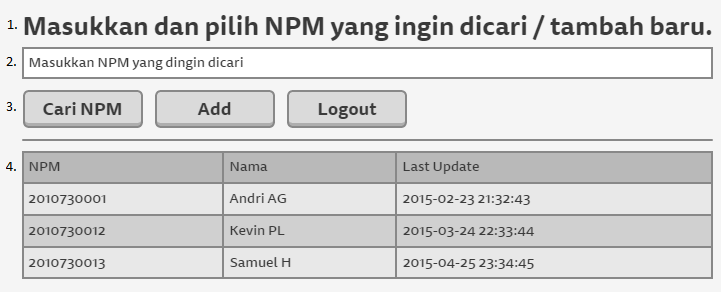
\includegraphics[scale=0.5]{Gambar/pilihmahasiswa.png}
\caption[Tampilan pilihmahasiswa.php Dengan Zurb Foundation]{Tampilan pilihmahasiswa.php Dengan Zurb Foundation} 
\label{fig:pilihmahasiswa}
\end{figure}

\section{Analisis Berorientasi Objek}
\label{sec:analisisberorientasiobjek}

Pembahasan use case diagram dan skenario yang akan digunakan pada penelitian.

\subsection{Use Case Diagram}
\begin{figure}[H]
\centering
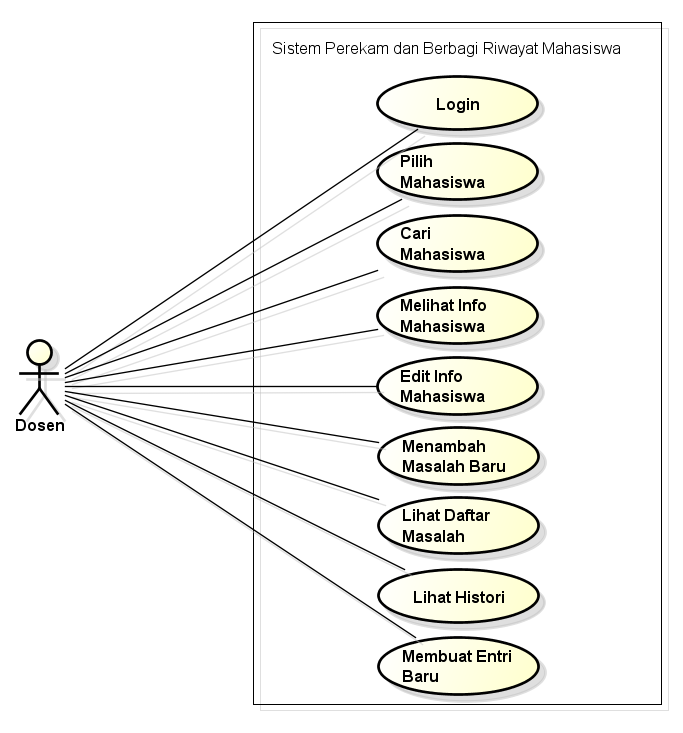
\includegraphics[scale=1]{Gambar/usecase.png}
\caption[Use Case Diagram]{Use Case Diagram} 
\label{fig:usecase}
\end{figure}

Use case diagram merupakan pemodelan yang menunjukkan kegiatan apa saja yang dapat dilakukan pengguna dan kegiatan yang dilakukan sistem. Berikut adalah deskripsi dari use case pada gambar \ref{fig:usecase}.

\begin{itemize}
\item Login\\
Use case ini memungkinkan pengguna untuk login via Google OAuth.
\item Pilih Mahasiswa\\
Use case ini memungkinkan pengguna untuk memilih mahasiswa yang ingin dilihat infonya. Selain itu pengguna juga bisa nemenkan tombol "Add" untuk menambah entri baru.
\item Melihat Info Mahasiswa\\
Use case ini memungkinkan pengguna untuk melihat info mahasiswa. Selain itu pengguna bisa menekan tombol "Edit" untuk mengedit info mahasiswa dan pengguna juga bisa menekan tombol "Lihat Histori" untuk melihat histori.
\item Edit Mahasiswa\\
Use case ini memungkinkan pengguna untuk mengedit info mahasiswa yang sudah ada.
\item Lihat Histori\\
Use case ini memungkinkan pengguna untuk melihat histori untuk setiap perubahan dan aksi view.
\item Membuat Entri Baru\\
Use case ini memungkinkan pengguna untuk membuat entri baru dengan memasukan inputan pada form yang telah disediakan.
\end{itemize}

\subsection{Skenario}
\subsubsection{Login}

\begin{table}
\centering
\caption[Tabel 3-1 Skenario Login]{Skenario Login}
\label{tab:skenariologin}
\begin{tabular}{|p{1.4cm}|p{0.4cm}|p{2cm}|p{2cm}|p{2cm}|p{2cm}|}
\hline
Nama & \multicolumn{5}{p{8cm}|}{Login} \\ \hline
Aktor & \multicolumn{5}{p{8cm}|}{Pengguna} \\ \hline
Deskripsi & \multicolumn{5}{p{8cm}|}{Melakukan login via Google OAuth} \\ \hline
Kondisi Awal & \multicolumn{5}{p{8cm}|}{Masih berada pada login.php} \\ \hline
Kondisi Akhir & \multicolumn{5}{p{8cm}|}{Sudah berada pada pilihmahasiswa.php} \\ \hline
\multirow{Skenario Utama} & No & \multicolumn{2}{p{4cm}|}{Aksi Aktor} & \multicolumn{2}{p{4cm}|}{Reaksi Sistem} \\ \cline{2-6} 
 & 1 & \multicolumn{2}{p{4cm}|}{Pengguna melakukan login} & \multicolumn{2}{p{4cm}|}{Server akan mengirimkan pertanyaan untuk izin} \\ \cline{2-6} 
 & 2 & \multicolumn{2}{p{4cm}|}{Pengguna memberikan izin} & \multicolumn{2}{p{4cm}|}{Aplilasi mendapatkan otorisasi kode} \\ \hline
Eksepsi & \multicolumn{5}{p{8cm}|}{Pengguna harus memiliki email yang diakhiri @unpar.ac.id dan username bukan angka semua} \\ \hline
\end{tabular}
\end{table}

Untuk use case Login, skenarionya dapat dilihat pada Tabel \ref{tab:skenariologin}.

\subsubsection{Pilih Mahasiswa}

\begin{table}
\centering
\caption[Tabel 3-2 Skenario Pilih Mahasiswa]{Skenario Pilih Mahasiswa}
\label{tab:skenariopilih}
\begin{tabular}{|p{1.4cm}|p{0.4cm}|p{2cm}|p{2cm}|p{2cm}|p{2cm}|}
\hline
Nama & \multicolumn{5}{p{8cm}|}{Pilih Mahasiswa} \\ \hline
Aktor & \multicolumn{5}{p{8cm}|}{Pengguna} \\ \hline
Deskripsi & \multicolumn{5}{p{8cm}|}{Pengguna dapat memilih dan mencari mahasiswa bedasarkan NPM} \\ \hline
Kondisi Awal & \multicolumn{5}{p{8cm}|}{Sebuah form dengan tabel yang berisi data mahasiswa} \\ \hline
Kondisi Akhir & \multicolumn{5}{p{8cm}|}{Salah satu mahasiswa terpilih} \\ \hline
\multirow{Skenario Utama} & No & \multicolumn{2}{p{4cm}|}{Aksi Aktor} & \multicolumn{2}{p{4cm}|}{Reaksi Sistem} \\ \cline{2-6} 
 & 1 & \multicolumn{2}{p{4cm}|}{Pengguna mencari mahasiswa berdasarkan NPM} & \multicolumn{2}{p{4cm}|}{Sistem seleksi mahasiswa berdasarkan NPM} \\ \cline{2-6} 
 & 2 & \multicolumn{2}{p{4cm}|}{Pengguna mengklik NPM mahasiswa yang dipilih} & \multicolumn{2}{p{4cm}|}{Pindah ke halaman infomahasiswa.php} \\ \hline
Eksepsi & \multicolumn{5}{p{8cm}|}{-} \\ \hline
\end{tabular}
\end{table}

Untuk use case Pilih Mahasiswa, skenarionya dapat dilihat pada Tabel \ref{tab:skenariopilih}.

\subsubsection{Melihat Info Mahasiswa}

\begin{table}
\centering
\caption[Tabel 3-3 Skenario Melihat Info Mahasiswa]{Skenario Melihat Info Mahasiswa}
\label{tab:skenarioinfo}
\begin{tabular}{|p{1.4cm}|p{0.4cm}|p{2cm}|p{2cm}|p{2cm}|p{2cm}|}
\hline
Nama & \multicolumn{5}{p{8cm}|}{Melihat Info Mahasiswa} \\ \hline
Aktor & \multicolumn{5}{p{8cm}|}{Pengguna} \\ \hline
Deskripsi & \multicolumn{5}{p{8cm}|}{Melihat info mahasiswa yang telah dipilih pada pilihmahasiswa.php} \\ \hline
Kondisi Awal & \multicolumn{5}{p{8cm}|}{Menampilkan info yang dimiliki mahasiswa} \\ \hline
Kondisi Akhir & \multicolumn{5}{p{8cm}|}{Jika pengguna mengklik "Edit" maka pindah ke editmahasiswa.php. Jika pengguna mengklik "Lihat Histori" maka pindah ke lihathistori.php} \\ \hline
\multirow{Skenario Utama} & No & \multicolumn{2}{p{4cm}|}{Aksi Aktor} & \multicolumn{2}{p{4cm}|}{Reaksi Sistem} \\ \cline{2-6} 
 & 1 & \multicolumn{2}{p{4cm}|}{Pengguna melihat info mahasiswa} & \multicolumn{2}{p{4cm}|}{Sistem menampilkan info mahasiswa} \\ \hline
Eksepsi & \multicolumn{5}{p{8cm}|}{-} \\ \hline
\end{tabular}
\end{table}

Untuk use case Melihat Info Mahasiswa, skenarionya dapat dilihat pada Tabel \ref{tab:skenarioinfo}.

\subsubsection{Edit Mahasiswa}

\begin{table}
\centering
\caption[Tabel 3-4 Skenario Edit Mahasiswa]{Skenario Edit Mahasiswa}
\label{tab:skenarioedit}
\begin{tabular}{|p{1.4cm}|p{0.4cm}|p{2cm}|p{2cm}|p{2cm}|p{2cm}|}
\hline
Nama & \multicolumn{5}{p{8cm}|}{Edit Mahasiswa} \\ \hline
Aktor & \multicolumn{5}{p{8cm}|}{Pengguna} \\ \hline
Deskripsi & \multicolumn{5}{p{8cm}|}{Mengedit info mahasiswa yang sudah ada di database} \\ \hline
Kondisi Awal & \multicolumn{5}{p{8cm}|}{Menampilkan form dengan data yang sudah ada pada database} \\ \hline
Kondisi Akhir & \multicolumn{5}{p{8cm}|}{Form dengan data yang telah diedit} \\ \hline
\multirow{Skenario Utama} & No & \multicolumn{2}{p{4cm}|}{Aksi Aktor} & \multicolumn{2}{p{4cm}|}{Reaksi Sistem} \\ \cline{2-6} 
 & 1 & \multicolumn{2}{p{4cm}|}{Pengguna mengedit data yang sudah ada} & \multicolumn{2}{p{4cm}|}{Sistem menampilkan data yang sudah ada} \\ \cline{2-6} 
 & 2 & \multicolumn{2}{p{4cm}|}{Pengguna menyimpan perubahan} & \multicolumn{2}{p{4cm}|}{Sistem akan merekan perubahan ke dalam database} \\ \hline
Eksepsi & \multicolumn{5}{p{8cm}|}{-} \\ \hline
\end{tabular}
\end{table}

Untuk use case Edit Mahasiswa, skenarionya dapat dilihat pada Tabel \ref{tab:skenarioedit}.

\subsubsection{Lihat Histori}

\begin{table}
\centering
\caption[Tabel 3-5 Skenario Lihat Histori]{Skenario Lihat Histori}
\label{tab:skenariohistori}
\begin{tabular}{|p{1.4cm}|p{0.4cm}|p{2cm}|p{2cm}|p{2cm}|p{2cm}|}
\hline
Nama & \multicolumn{5}{p{8cm}|}{Lihat Histori} \\ \hline
Aktor & \multicolumn{5}{p{8cm}|}{Pengguna} \\ \hline
Deskripsi & \multicolumn{5}{p{8cm}|}{Melihat histori perubahan dan aksi melihat yang dilakukan pengguna} \\ \hline
Kondisi Awal & \multicolumn{5}{p{8cm}|}{Menampilkan log histori perubahan dan aksi melihat} \\ \hline
Kondisi Akhir & \multicolumn{5}{p{8cm}|}{Terus bertambah sesuai aksi yang dilakukan} \\ \hline
\multirow{Skenario Utama} & No & \multicolumn{2}{p{4cm}|}{Aksi Aktor} & \multicolumn{2}{p{4cm}|}{Reaksi Sistem} \\ \cline{2-6} 
 & 1 & \multicolumn{2}{p{4cm}|}{Pengguna melihat log histori} & \multicolumn{2}{p{4cm}|}{Sistem akan menampilkan loh hisotri} \\ \hline
Eksepsi & \multicolumn{5}{p{8cm}|}{-} \\ \hline
\end{tabular}
\end{table}

Untuk use case Lihat Histori, skenarionya dapat dilihat pada Tabel \ref{tab:skenariohistori}.

\subsubsection{Membuat Entri Baru}

\begin{table}
\centering
\caption[Tabel 3-6 Skenario Membuat Entri Baru]{Skenario Membuat Entri Baru}
\label{tab:skenarioentribaru}
\begin{tabular}{|p{1.4cm}|p{0.4cm}|p{2cm}|p{2cm}|p{2cm}|p{2cm}|}
\hline
Nama & \multicolumn{5}{p{8cm}|}{Membuat Entri Baru} \\ \hline
Aktor & \multicolumn{5}{p{8cm}|}{Pengguna} \\ \hline
Deskripsi & \multicolumn{5}{p{8cm}|}{Membuat entri baru yang belum ada pada database} \\ \hline
Kondisi Awal & \multicolumn{5}{p{8cm}|}{Menampilkan form untuk menambah entri baru} \\ \hline
Kondisi Akhir & \multicolumn{5}{p{8cm}|}{Input pada form akan dimasukan kedalam database} \\ \hline
\multirow{Skenario Utama} & No & \multicolumn{2}{p{4cm}|}{Aksi Aktor} & \multicolumn{2}{p{4cm}|}{Reaksi Sistem} \\ \cline{2-6} 
 & 1 & \multicolumn{2}{p{4cm}|}{Pengguna mengisi form entri baru} & \multicolumn{2}{p{4cm}|}{Sistem menampilkan form entri baru} \\ \cline{2-6} 
 & 2 & \multicolumn{2}{p{4cm}|}{Pengguna menyimpan inputan dari form entri baru} & \multicolumn{2}{p{4cm}|}{Sistem akan merekan inputan pengguna ke dalam database} \\ \hline
Eksepsi & \multicolumn{5}{p{8cm}|}{-} \\ \hline
\end{tabular}
\end{table}

Untuk use case Membuat Entri Baru, skenarionya dapat dilihat pada Tabel \ref{tab:skenarioentribaru}.